
    \begin{frame}{Balance}

      The number of $x \equiv i \mod v$ in $[1,p-1]$ is
      \[ \lceil (p-1 - ((i-1) \bmod v))/v\rceil\]

\begin{proposition} \label{balancedproperty}
Let $\pi$ be a permutation in $\zpx$, then $\pi_v$ is a balanced 
sequence over $\z_v$ if and only if $v \mid p-1$.
\end{proposition}
      
      \end{frame}


      \begin{frame}{Period}

        \begin{lemma} \label{lemma_near_balanced_period}
If $p \equiv \alpha \neq 1 \Mod v$, then $\pi_v$ has period $N =p-1$ for any $\pi: \zpx \rightarrow \zpx$.
\end{lemma}
\begin{proof}

  The difference in the number of occurences of any two symbols must be a multiple of $(p-1)/N$. But   
  \[
    |\pi_v|_a = \begin{cases} \lceil (p-1)/v \rceil &  0 \leq a < \alpha -1, \\
      \lfloor (p-1)/v \rfloor & \mbox{otherwise}.
    \end{cases}
  \]
\end{proof}

\end{frame}

\begin{frame}{Period}


\begin{theorem}For every $\epsilon >0 $ there exists an $n_{\epsilon}$ so that for 
  all $p \geq n_{\epsilon}$, the number $T$ of permutations $\pi_v$ with period 
  $p-1$ satisfies 
  \begin{equation} \label{T_bound_epsilon}
    (p-1)!(1-\epsilon) \leq T \leq (p-1)!.
  \end{equation}
\end{theorem}
  
\end{frame}


\begin{frame}{Special case}

  When $q$ is prime and $p=vq+1$,
  \[
    (p-1)! - T = v!(q!)^v 
    \]

    This includes the case of Sophie Germain primes.
  
  \end{frame}

  \begin{frame}{de Bruijn graph}
    \usetikzlibrary {arrows.meta}
    \begin{center}
      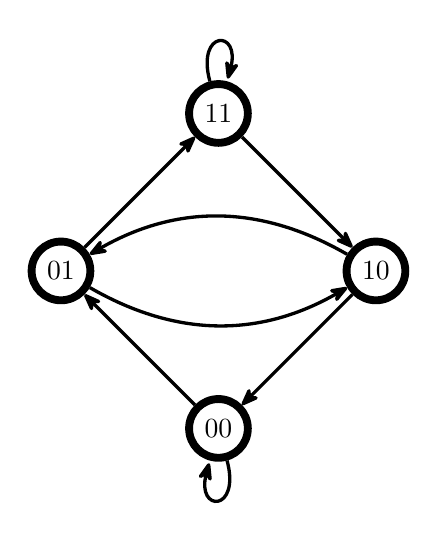
\begin{tikzpicture}
%        [->,>={Stealth[round]},shorten >=1pt,auto,node distance=2.8cm,on grid,semithick]
        [->,>={Stealth[round]},auto,node distance=2.8cm,very thick]
      \node (00) at  (0,0) [circle,draw=black,line width=1.0mm] {00};
      \node (01) at  (-2,2) [circle,draw=black,line width=1.0mm] {01};
      \node (10) at  (2,2) [circle,draw=black,line width=1.0mm] {10};
      \node (11) at  (0,4) [circle,draw=black,line width=1.0mm] {11};

      \path (00) edge [loop below] (00);
      \path (00) edge (01);
      \path (10) edge (00);
      \draw (10) to[out=150,in=30]  (01);
      \draw (01) to[out=-30,in=-150]  (10);
      \path (01) edge (11);
      \path (11) edge (10);
      \path (11) edge [loop above] (11);
    \end{tikzpicture}
    \end{center}

  \end{frame}

  \begin{frame}{Transfer Matrix}


    
    Transfer matrix is directed adjacency matrix of de Bruijn graph with variables
    \[
      T =  \bordermatrix{ & 00 & 01 & 10 & 11 \cr
     00 & ux_0 & ux_0 & 0 & 0 \cr
     01 & 0 & 0 & x_0 & x_0 \cr
     10 & 1 & 1 & 0 & 0\cr
   11 & 0 & 0 & 1 & 1}
      \]

\[
      C =  \bordermatrix{ & 00 & 01 & 10 & 11 \cr
     00 & 1 & 0 & 0 & 0 \cr
     01 & 0 & 1 & 0 & 0 \cr
     10 & 0 & 0 & 1 & 0\cr
   11 & 0 & 0 & 0 & 1}
      \]

\[
  \sum_{\mathbf{k} \in \mathbb{N}^t} a_n(k)x^{\mathbf k} = \sum_{z',z'' \in \z_v^t} C_{z',z''} T^{n}_{z',z''}.
\]
      
\end{frame}


 	

%%% Local Variables:
%%% TeX-master: "../main.tex"
%%% End:
